\section{Concept Learning}
\label{sec:appendix-A}
\subsection{Connection to the Bhattacharya Distance}
\label{sec:appendix-BC-distance}
We note that the proposed separability metric in Section \ref{sec:separability_score} is closely related to the Bhattacharya distance~\cite{bhattacharyya1943measure} for the special case when the concept scores from both ID and OOD data follow a multivariate Gaussian density. The Bhattacharya distance is a well known measure of divergence between two probability distributions, and it has the nice property of being an upper bound to the Bayes error rate in the two-class case~\cite{fukunaga1990bhatta}. For the special case when the concept scores from both ID and OOD data follow a multivariate Gaussian with a shared covariance matrix, it can be shown that the Bhattacharya distance reduces to the following separability metric (ignoring scale factors): 
\begin{align}
\label{eq:separability_trace}
&J_{\textrm{sep}}(\bfC) ~:=~ J_{\textrm{sep}}(V_{\textrm{in}}(\bfC), V_{\textrm{out}}(\bfC)) ~=~ \textrm{tr}\big[\bfS_w^{-1} \,\bfS_b\big].
%
% &=~ \textrm{tr}\big[\bfS_w^{-1} \,(\bfmu_{\textrm{out}} \,-\, \bfmu_{\textrm{in}})\,(\bfmu_{\textrm{out}} \,-\, \bfmu_{\textrm{in}})^T\big] \nonumber \\
%
% &=~ (\bfmu_{\textrm{out}} \,-\, \bfmu_{\textrm{in}})^T \,\bfS_w^{-1} \,(\bfmu_{\textrm{out}} \,-\, \bfmu_{\textrm{in}}).
\end{align}

\iffalse

We sometimes denote $J_{\textrm{sep}}(V_{\textrm{in}}(\bfC), V_{\textrm{out}}(\bfC))$ as $J_{\textrm{sep}}(\bfC)$ for brevity.
Assumption of unimodal distribution; when this assumption may not be appropriate in some cases. 
\fi

\subsection{Per-class Detection Completeness}
\label{sec:appendix-perclass-completeness}
We propose a per-class measure for the detection completeness (denoted by $\eta^{y}_{\bff, S}(\bfC)$), which is obtained by simply modifying $\eta^{}_{\bff, S}(\bfC)$ in Eqn. (\ref{equ: completeness-detection}) based on the subset of ID and OOD data that are predicted into class $y \in [L]$ by the classifier.
% One can simply compute Eqn. (\ref{equ: completeness-detection}) and Eqn. (\ref{eq:separability_trace}) using the subset of ID and OOD data whose predictions are class $y \in [L]$. 
% We refer to this per-class variation as the \textit{per-class detection completeness} (denoted by $\eta^{y}_{\bff, S}(\bfC)$).

\begin{definition}
\label{def:completeness_detec_perclass}
Given a trained DNN classifier $\bff = \bfh \circ \bfphi$, a trained OOD detector with score function $S(\bfx, \bff)$, and a set of concept vectors $\bfC$, the {\em per-class detection completeness} relative to class $y \in [L]$ with respect to the ID distribution $\Pin(\bfx, y)$ and OOD distribution $\Pout(\bfx)$ is defined as
\begin{align}
\label{equ: completeness-detection-perclass}
    \eta^{y}_{\bff, S}(\bfC) 
    ~:=~ \frac{\textrm{sup}_\bfg \,\textrm{AUC}^y(\bfh \circ \recphi) ~-~ b_r}{\textrm{AUC}(\bfh \circ \bfphi) ~-~ b_r},
\end{align}
\end{definition}
where $\textrm{AUC}^y(\bfh \circ \recphi)$ is the AUROC of the detector conditioned on the event that the class predicted by the concept-world classifier $\,\bfh \circ \recphi\,$ is $y$. We note that the denominator in the above metric is still the global AUROC. The baseline AUROC $b_r$ is equal to $0.5$.
This per-class detection completeness is used in the modified Shapley value defined in Section \ref{sec:expt_concept_based_explanations}.

\subsection{Per-class Concept Separability}
\label{sec:appendix-perclass-separability}
In section \ref{sec:separability_score}, we focused on the separability between the concept scores of ID and OOD data without considering the class prediction of the classifier.
However, it would be more appropriate to impose a high separability between the concept scores on a per-class level. In other words, we would like the concept scores of detected-ID and detected-OOD data, that are predicted by the classifier into any given class $y \in [L]$ to be well separated.
Consider the set of concept-score vectors from the detected-ID (or detected-OOD) dataset that are also predicted into class $y$:
\begin{align}
V^{y}_{\textrm{in}}(\bfC) ~&:=~ \{\TVC(\bfx), ~\bfx \in \Dintr \cup \Douttr ~:~ \calD_\gamma(\bfx, \bff) = 1~ \text{ and } ~\widehat{y}(\bfx) = y\} \nonumber \\
%
V^{y}_{\textrm{out}}(\bfC) ~&:=~ \{\TVC(\bfx), ~\bfx \in \Dintr \cup \Douttr ~:~ \calD_\gamma(\bfx, \bff) = 0~ \text{ and } ~\widehat{y}(\bfx) = y\}.
\end{align}
We can extend the definition of the global separability metric in Eq. (\ref{eq:separability_trace}) to a given predicted class $y \in [L]$ as follows
\begin{align}
\label{eq:separability_trace_per_class}
J^y_{\textrm{sep}}(\bfC) ~&:=~ J_{\textrm{sep}}(V^{y}_{\textrm{in}}(\bfC), V^{y}_{\textrm{out}}(\bfC)) ~=~ \textrm{tr}\big[(\bfS^{y}_w)^{-1} \,\bfS^y_b\big] \nonumber \\
&=~ (\bfmu^y_{\textrm{out}} \,-\, \bfmu^y_{\textrm{in}})^T \,(\bfS^y_w)^{-1} \,(\bfmu^y_{\textrm{out}} \,-\, \bfmu^y_{\textrm{in}}).
\end{align}
We refer to these per-class variations as \textit{per-class concept separability}.
The scatter matrices $\bfS^y_w$ and $\bfS^y_b$ are defined similar to Eq. (\ref{eq:scatter_matrices}), using the per-class subset of concept scores $V^{y}_{\textrm{in}}(\bfC)$ or $V^{y}_{\textrm{out}}(\bfC)$, and the mean concept-score vectors from the detected-ID and detected-OOD dataset are also defined at a per-class level.

% Ideally, a high global concept separability would ensure that on a macro level the concepts provide clear explanations regardless of the class and decision of the classifier. But, since the goal is to provide concept explanations for OOD detectors, we could still provide meaningful explanations on a per-class basis if we can separate out concepts that are from an OOD input classified as a certain class $c$, versus an ID input classified as $c$. Examining both metrics can help us gauge the relative separability on finer and coarser scales to evaluate the quality of the concept explanations.

\subsection{Algorithm for Concept Learning}
\label{sec:appendix-algo}
To provide the readers with a clear overview of the proposed concept learning approach, we include Algorithm \ref{alg:concept_learning}.
Note that in line 7 of Algorithm \ref{alg:concept_learning}, the dimension reduction step in $\,V_{\textrm{in}}(\bfC) = \{\TVC(\bfx), ~\bfx \in \Dintr \cup \Douttr ~:~ \calD_\gamma(\bfx, \bff) = 1\}\,$ and $\,V_{\textrm{out}}(\bfC) = \{\TVC(\bfx), ~\bfx \in \Dintr \cup \Douttr ~:~ \calD_\gamma(\bfx, \bff) = 0\}\,$ involves the maximum function, which is not differentiable; specifically, the step $\,\widetilde{v}_{\bfc_i}(\bfx) = \max_{p, q} |\langle \bfphi^{p,q}(\bfx), \bfc_i \rangle|$.
For calculating the gradients (backward pass), we use the \texttt{log-sum-exp} function with a temperature parameter to get a differentiable approximation of the maximum function, \ie $\max_{p, q} |\langle \bfphi^{p,q}(\bfx), \bfc_i \rangle| \,\approx\, \alpha \,\log \left[ \sum_{p,q} \exp\left( \frac{1}{\alpha} \,|\langle \bfphi^{p,q}(\bfx), \bfc_i \rangle| \right) \right]\,$ as $\alpha \rightarrow 0$.
In our experiments, we set the temperature constant $\alpha = 0.001$ upon checking that the approximate value of $\,\widetilde{v}_{\bfc_i}(\bfx)$ is sufficiently close to the original value using the maximum function.

\begin{algorithm}[ht]
\caption{Learning concepts for OOD detector}
\label{alg:concept_learning}
\textbf{INPUT:} Entire training set $\Dtr = \{\Dintr, \Douttr\}$, entire validation set $\Dval = \{\Dinval, \Doutval\}$, classifier $\bff$, detector $\calD_\gamma$. \\
\textbf{INITIALIZE:} Concept vectors $\bfC = [\bfc_1 \cdots \bfc_m]$ and parameters of the network $\bfg$. \\
\textbf{OUTPUT:} $\bfC$ and $\bfg$.
\begin{algorithmic}[1]
  \STATE Calculate threshold $\gamma$ for $\calD_\gamma$ using $\Dval$ as the score at which true positive rate is $95\%$.
%   , and prepare $\widehat{\Dinval}$ and $\widehat{\Doutval}$;
  \FOR{$t = 1, ... T$ epochs}
    \STATE Compute the prediction accuracy of the concept-world classifier $\fcon$ using $\Dintr$.
    \STATE Compute the explainability regularization term as defined in \cite{yeh2020completeness}.
	\STATE Compute difference of feature representation between canonical world and concept world (i.e. $J_{\textrm{norm}}(\bfC, \bfg)$).
	% Compute the squared-norm regularization term using Eqn. (\ref{equ:regularizer_norm}).
	\STATE Compute difference of detector outputs between canonical world and concept world using Eqn. (\ref{equ:regularizer_mse}).
% 	\STATE Compute $V_{\textrm{in}}(\bfC)$~\footnotemark{} and $V_{\textrm{out}}(\bfC)$ using $\Dtr, \calD_\gamma$ and $\bfC$.
	\STATE Compute $V_{\textrm{in}}(\bfC)$ and $V_{\textrm{out}}(\bfC)$ using $\Dtr, \calD_\gamma$ and $\bfC$.
	\STATE Compute separability between $V_{\textrm{in}}(\bfC)$ and $V_{\textrm{out}}(\bfC)$ using Eqn. (\ref{eq:separability_trace}) or Eqn. (\ref{eq:separability_trace_per_class}).
    \STATE Perform a batch-SGD update of $\bfC$ and $g$ using Eqn. (\ref{equ: concept learning}) as the objective.
  \ENDFOR
\end{algorithmic} 
\end{algorithm}
% \footnotetext{To make the dimension reduction step in $V_{\textrm{in}}(\bfC) := \{\widetilde{v}_{\bfc_i}(\bfx) ~|~ \widetilde{v}_{\bfc_i}(\bfx) = \max_{p, q} |\langle \bfphi^{p,q}(\bfx), \bfc_i \rangle|, \, \bfx \sim \Pin\} $ differentiable, we take a smooth approximation of the maximum function using the \texttt{log-sum-exp} function: $\max_{p, q} |\langle \bfphi^{p,q}(\bfx), \bfc_i \rangle| \approx \frac{1}{\alpha}\sum_{p,q}\log(e^{\alpha |\langle \bfphi^{p,q}(\bfx), \bfc_i \rangle|})\,$ as $\alpha \rightarrow \infty$. The same approximation is applied to $V_{\textrm{out}}(\bfC)$.}


\iffalse
\subsection{Concept separability and visual distinction in explanations}

\begin{figure}
  \centering
  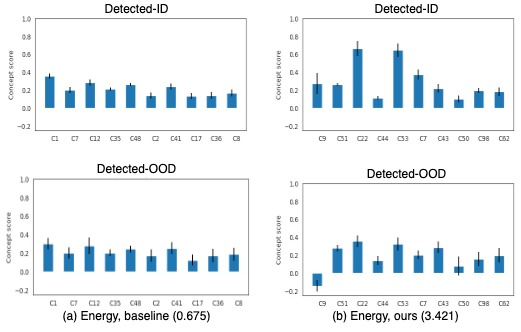
\includegraphics[width=0.8\linewidth]{figures/visual_dstinct.jpg}
  \captionof{figure}{
\small \textbf{Concept separability and visual distinction in the concept score patterns.} For the class "Giraffe", we compare the concept score patterns using two different sets of concepts. \textbf{Left:} Averaged scores of top-10 important concepts out of the concepts learned by ~\cite{yeh2020completeness}). 
\textbf{Right:} Averaged scores of top-10 important concepts out of the concepts learned by our method ($\,\lambda_\textrm{mse} = 1, \lambda_\textrm{norm} = 0.1, \lambda_\textrm{sep} = 50$ with Energy detector).
Concept importance is measured using the Shapley value of Eqn. (\ref{equ: ConceptSHAP}).
% For visualization of what each concept represents, see Appendix.
% C$i$ denotes $i$-th concept.
}
\label{fig:separa_interpretatbility}
\end{figure}

% Lastly, we use the concepts to gain insights on OOD detectors.
% We investigate whether the concepts with a higher concept-separability measure lead to a more distinguishable pattern 
%in the concept scores between detected-ID inputs and detected-OOD inputs. 
% between the concept scores of detected-ID inputs and detected-OOD inputs.
In Fig. \ref{fig:separa_interpretatbility}, we take the average of concept scores $V_{\textrm{in}}(\bfC)$ (or $V_{\textrm{out}}(\bfC)$) among the inputs that are predicted as class $y$, and detected as ID (or OOD) by Energy detector as an example.
% where $\bfC'$ is the subset of original $m$ concepts $\bfC$. 
% Here, we constitute the subset by taking the top-10 important concepts, ranked by their SHAP($\eta^{j}_{\bff, S}(\bfC)$) scores.
% By comparing the patterns of averaged concept scores, one can understand how ID-detected inputs and OOD-detected inputs are different in terms of concepts, even when predicted to same class (compare Figure \ref{fig:low_in} vs. Figure \ref{fig:low_out}, or Figure \ref{fig:high_in} vs. Figure \ref{fig:high_out}).
We can observe noticeably distinguishable pattern between detected-ID and detected-OOD concept scores when using concepts with higher concept separability ($J_{\textrm{sep}}(\bfC, \bfC')=3.421$), compared to those of low concept separability ($J_{\textrm{sep}}(\bfC, \bfC')=0.675$) by ~\cite{yeh2020completeness}. 
These observations confirm our design motivation for the concept separability metric -- that a higher value of the concept separability metric enables better \textit{visual distinction} between the concept score patterns, suggesting better interpretability for humans.
%This suggests that as long as classification completeness and detection completeness are preserved, having higher concept separability is beneficial for better interpretability for humans. 
% For further discussion, see Appendix \ref{sec:appendix-separability}.
\fi